\section{Introduction}
\label{sec:introduction}

Cloud computing has revolutionized data storage and processing, offering on-demand access to vast computational resources without direct user management. However, the current landscape is dominated by a few major providers, leading to concerns about vendor lock-in, security vulnerabilities, and resource inefficiencies.

This paper presents a novel decentralized cloud platform that addresses these challenges while leveraging the strengths of both centralized and decentralized models. Our approach combines the reliability and performance of traditional cloud services with the flexibility and democratization of decentralized systems, creating a more robust, efficient, and user-centric cloud computing ecosystem.
\subsection{Background and Motivation}
\label{sec:background}

In response to these challenges, decentralized cloud computing has emerged as a promising alternative. This approach distributes data and processes across multiple machines, or nodes, each equipped with its own processing power and storage. This distribution can lead to more efficient resource allocation and utilization, as resources can be dynamically shared among nodes based on demand.

Our objective is to address the inherent issues of centralized cloud computing by constructing a secure and trustworthy system. This is achieved through the implementation of robust security measures and a reputation system, which collectively enhance the reliability and integrity of the platform.

Furthermore, we aim to promote transparency and democratic principles within the system by employing a decentralized matching engine and a Decentralized Autonomous Organization (DAO) model for governance. This approach is intended to stimulate competition and innovation in the field.

By lowering the barriers to becoming a cloud provider and offering a global rating system for all cloud providers, we enable developers to select providers based on their specific needs and preferences. This approach not only fosters a more competitive and innovative environment but also empowers developers by providing them with more choice and control over their cloud computing solutions.

\subsection{Academic research}

Decentralized cloud computing has garnered significant attention in the academic community as a viable alternative to centralized cloud models. Research in this domain explores various approaches to enhancing the efficiency, security, and scalability of cloud services through decentralization.

Xu Chen's work on "Decentralized Computation Offloading Game for Mobile Cloud Computing" \cite{chen2014decentralized} proposes a game-theoretic framework for efficient computation offloading in mobile cloud environments. This work highlights the potential of decentralized models in optimizing resource allocation, particularly in scenarios involving mobile devices with limited computational capabilities.
Similarly, Sladana Jošilo and G. Dán in their paper "Selfish Decentralized Computation Offloading for Mobile Cloud Computing in Dense Wireless Networks" \cite{josilo2018selfish} investigate the dynamics of decentralized computation offloading in dense wireless networks. Their research underscores the challenges of coordinating decentralized nodes and the importance of incentive mechanisms in ensuring efficient resource sharing.

Kunal et al.~\cite{kunal2019overview} explore fog computing as a decentralized layer between users and cloud servers, aiming to reduce latency and enhance service delivery. This research aligns with the broader goal of decentralization by distributing computational tasks closer to the edge, thereby improving responsiveness and reducing the load on central servers.

Nguyen et al.~\cite{nguyen2020integration} provide a comprehensive review of integrating blockchain with Cloud of Things (CoT), emphasizing the potential of blockchain to address decentralization challenges, enhance data privacy, and secure network transactions. Their work provides insights into the benefits of combining blockchain technology with decentralized cloud architectures.

Wenjuan Li et al. proposed a blockchain-based trust management system in cloud computing \cite{li2021blockchain}, which aligns closely with our platform's reputation-based approach. Their research illustrates how blockchain can be leveraged to establish trust among decentralized nodes, ensuring reliable and secure service delivery.

Chegini et al.~\cite{chegini2021process} discuss the automation of tasks and processes in the IoT-Fog-Cloud ecosystem, addressing big data and heterogeneity challenges. Their work highlights the need for decentralized solutions to manage the complexity and scale of modern cloud environments effectively.

Finally, Espinel Sarmiento et al.~\cite{sarmiento2021decentralized} survey the application of Software Defined Networks (SDN) in managing distributed Cloud-Edge infrastructures. This research is particularly relevant to our platform, as it demonstrates how SDN can facilitate the coordination and management of decentralized resources across a distributed cloud environment.

\subsection{Industry projects}

In recent years, several industry projects have attempted to build decentralized cloud platforms. These platforms leverage blockchain technology to create a network of independent node providers that can store data or run arbitrary workloads in a decentralized fashion, and highly resilient to malicious actors.

\begin{itemize}
    \item {\bf Filecoin} (\url{https://filecoin.io/}): Filecoin is a decentralized storage network designed to store and retrieve data in a distributed fashion. By incentivizing storage providers through its native cryptocurrency, Filecoin creates a competitive marketplace for data storage. While Filecoin excels in decentralized storage, it does not extend to compute resources. In contrast, our platform aims to integrate both storage and compute capabilities, offering a more holistic cloud solution.

    \item {\bf Storj} (\url{https://www.storj.io/}): Storj is a decentralized cloud storage platform that focuses on secure and distributed data storage. It fragments and encrypts data before distributing it across its network, ensuring high levels of security and redundancy. Similar to Filecoin, Storj is storage-centric and does not offer compute resources. Our platform distinguishes itself by providing a marketplace that includes both storage and compute services.

    \item {\bf Sia} (\url{https://sia.tech/}): Sia operates as a decentralized storage platform that leverages global hard drive capacity to create a distributed data storage network. While Sia effectively reduces storage costs and enhances data redundancy, it lacks the ability to offer compute resources. Additionally, it does not incorporate a reputation-based system for node providers. Our platform addresses these gaps by integrating compute capabilities and establishing a reputation system to enhance trust and reliability.

    \item {\bf Arweave} (\url{https://www.arweave.org/}): Arweave offers a unique approach to data storage by providing permanent and sustainable storage solutions. It is particularly suited for archiving and storing immutable data. However, Arweave's focus on storage limits its applicability in scenarios requiring compute resources. Our platform expands on this by supporting both storage and compute, catering to a broader range of cloud computing needs.

    \item {\bf DFINITY} (\url{https://dfinity.org/}): DFINITY's Internet Computer represents a significant step toward decentralized cloud computing by enabling developers to host entire applications on its decentralized network. Despite its innovation, the Internet Computer's reliance on the Consensus protocol imposes performance limitations, particularly for high-throughput applications. Our platform, by contrast, separates the control and data planes, allowing for higher performance and broader applicability across diverse workloads.

    \item {\bf Akash Network} (\url{https://akash.network/}): Akash Network is a decentralized cloud computing platform that focuses on offering compute resources through a permissionless marketplace. Akash allows users to rent computing power from providers across the globe, targeting workloads such as web hosting, machine learning, and containerized applications. While Akash shares similarities with our platform, our solution emphasizes a more comprehensive approach, integrating robust reputation systems and legal frameworks to ensure quality and reliability, which many users see as essential.

    \item {\bf Golem} (\url{https://golem.network/}): Golem functions as a decentralized supercomputer that aggregates the computational power of user machines worldwide. It is particularly well-suited for compute-intensive tasks such as rendering and scientific simulations. However, Golem's focus on specialized compute tasks limits its versatility as a general-purpose cloud platform. Our platform aims to provide a more flexible solution that accommodates a wide range of workloads, from basic web hosting to complex AI processing.

    \item {\bf iExec} (\url{https://iex.ec/}): iExec provides a decentralized marketplace for cloud computing resources, primarily serving decentralized applications (DApps) on blockchain networks. While iExec offers an efficient solution for DApp developers, its reliance on the Consensus protocol can slow down execution times, limiting its use for performance-sensitive applications. Our platform, by contrast, is designed to serve a broader spectrum of applications, with a focus on minimizing latency and maximizing performance.

    \item {\bf Aethir} (\url{https://www.myedge.io/}): Aethir offers a decentralized marketplace for renting GPU resources, specifically targeting machine learning (ML) and artificial intelligence (AI) workloads. By focusing on GPU availability, Aethir addresses a critical need in the AI and ML communities. Our platform incorporates similar GPU rental capabilities but extends the offering to include other compute and storage resources, providing a more comprehensive cloud solution.

    \item {\bf Cudos} (\url{https://www.cudos.org/}): Cudos is a decentralized cloud computing platform that aims to bridge the gap between cloud and blockchain by providing compute resources for blockchain and non-blockchain applications. Cudos supports a wide range of workloads, from simple hosting to complex decentralized finance (DeFi) applications. Our platform builds on these ideas by offering an even more integrated approach, combining compute, storage, and reputation systems within a single ecosystem.

    \item {\bf ICN (Impossible Cloud Network)} (\url{https://icn.global/}): The Impossible Cloud Network (ICN) is a decentralized approach to cloud infrastructure, providing a platform for managing hardware and cloud resources. It leverages decentralized technologies to ensure data security, integrity, and resiliency. ICN's approach to managing global cloud resources aligns with our platform's goal of mitigating vendor lock-in while enhancing transparency and control. Our platform further differentiates itself by integrating a reputation system and legal frameworks to ensure service quality and compliance.

    \item {\bf Fluence} (\url{https://fluence.dev/}): Fluence offers a decentralized serverless platform that enables developers to deploy applications without the need for centralized servers. It provides a peer-to-peer network for executing code, using a special-purpose language called Aqua for cryptographic proofs. While Fluence's approach is innovative, the need for specialized language limits its flexibility. Our platform, in contrast, supports a broader range of programming languages and environments, and integrates a reputation system to ensure service quality and compliance, making it accessible to a wider audience and a wider range of use cases.
\end{itemize}

These works highlight the growing interest in decentralized cloud computing and the potential benefits it can offer.
However, despite these efforts there is still a need for a comprehensive solution that addresses the issues of the current cloud computing paradigm while leveraging the benefits of decentralization. This is the problem that our proposed decentralized cloud platform aims to solve and in the following sections we provide an outline of how we plan to do this.

\begin{figure*}[ht]
    \centering
    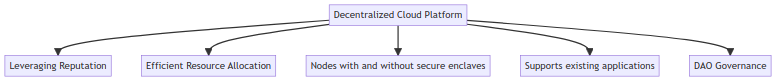
\includegraphics[width=\textwidth]{figures/proposed-solution.png}
    \caption{An illustration of the proposed solution.}
\end{figure*}
